% Created by tikzDevice version 0.12.6 on 2026-08-08 12:10:30
% !TEX encoding = UTF-8 Unicode
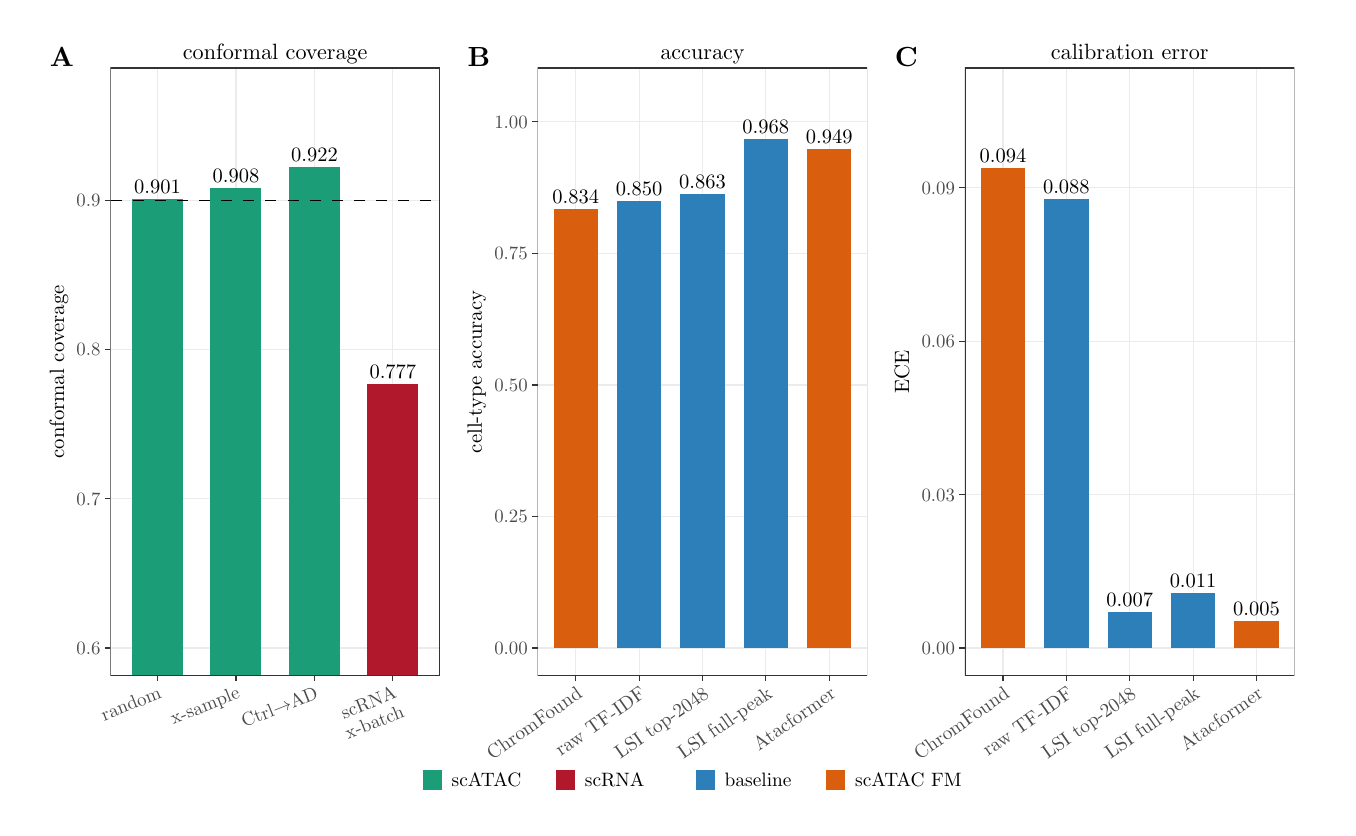
\begin{tikzpicture}[x=1pt,y=1pt]
\definecolor{fillColor}{RGB}{255,255,255}
\path[use as bounding box,fill=fillColor,fill opacity=0.00] (0,0) rectangle (469.75,281.85);
\begin{scope}
\path[clip] (  0.00,  0.00) rectangle (469.75,281.85);
\definecolor{drawColor}{RGB}{255,255,255}
\definecolor{fillColor}{RGB}{255,255,255}

\path[draw=drawColor,line width= 0.4pt,line join=round,line cap=round,fill=fillColor] ( -0.00,  0.00) rectangle (469.76,281.85);
\end{scope}
\begin{scope}
\path[clip] (  4.00,  3.00) rectangle (154.99,278.85);
\definecolor{drawColor}{RGB}{255,255,255}
\definecolor{fillColor}{RGB}{255,255,255}

\path[draw=drawColor,line width= 0.4pt,line join=round,line cap=round,fill=fillColor] (  4.00,  3.00) rectangle (154.99,278.85);
\end{scope}
\begin{scope}
\path[clip] (154.99,  3.00) rectangle (309.37,278.85);
\definecolor{drawColor}{RGB}{255,255,255}
\definecolor{fillColor}{RGB}{255,255,255}

\path[draw=drawColor,line width= 0.4pt,line join=round,line cap=round,fill=fillColor] (154.99,  3.00) rectangle (309.37,278.85);
\end{scope}
\begin{scope}
\path[clip] (309.37,  3.00) rectangle (463.75,278.85);
\definecolor{drawColor}{RGB}{255,255,255}
\definecolor{fillColor}{RGB}{255,255,255}

\path[draw=drawColor,line width= 0.4pt,line join=round,line cap=round,fill=fillColor] (309.37,  3.00) rectangle (463.75,278.85);
\end{scope}
\begin{scope}
\path[clip] ( 29.91, 47.70) rectangle (148.99,267.29);
\definecolor{fillColor}{RGB}{255,255,255}

\path[fill=fillColor] ( 29.91, 47.70) rectangle (148.99,267.29);
\definecolor{drawColor}{gray}{0.92}

\path[draw=drawColor,line width= 0.4pt,line join=round] ( 29.91, 57.68) --
	(148.99, 57.68);

\path[draw=drawColor,line width= 0.4pt,line join=round] ( 29.91,111.63) --
	(148.99,111.63);

\path[draw=drawColor,line width= 0.4pt,line join=round] ( 29.91,165.59) --
	(148.99,165.59);

\path[draw=drawColor,line width= 0.4pt,line join=round] ( 29.91,219.54) --
	(148.99,219.54);

\path[draw=drawColor,line width= 0.4pt,line join=round] ( 46.92, 47.70) --
	( 46.92,267.29);

\path[draw=drawColor,line width= 0.4pt,line join=round] ( 75.27, 47.70) --
	( 75.27,267.29);

\path[draw=drawColor,line width= 0.4pt,line join=round] (103.62, 47.70) --
	(103.62,267.29);

\path[draw=drawColor,line width= 0.4pt,line join=round] (131.97, 47.70) --
	(131.97,267.29);
\definecolor{fillColor}{RGB}{27,158,119}

\path[fill=fillColor] ( 37.71,-266.04) rectangle ( 56.14,220.03);

\path[fill=fillColor] ( 66.06,-266.04) rectangle ( 84.49,223.91);

\path[fill=fillColor] ( 94.41,-266.04) rectangle (112.84,231.46);
\definecolor{fillColor}{RGB}{178,24,43}

\path[fill=fillColor] (122.76,-266.04) rectangle (141.19,153.18);
\definecolor{drawColor}{RGB}{0,0,0}

\path[draw=drawColor,line width= 0.4pt,dash pattern=on 4pt off 4pt ,line join=round] ( 29.91,219.54) -- (148.99,219.54);

\node[text=drawColor,anchor=base,inner sep=0pt, outer sep=0pt, scale=  0.74] at ( 46.92,222.06) {0.901};

\node[text=drawColor,anchor=base,inner sep=0pt, outer sep=0pt, scale=  0.74] at ( 75.27,225.95) {0.908};

\node[text=drawColor,anchor=base,inner sep=0pt, outer sep=0pt, scale=  0.74] at (103.62,233.50) {0.922};

\node[text=drawColor,anchor=base,inner sep=0pt, outer sep=0pt, scale=  0.74] at (131.97,155.22) {0.777};
\definecolor{drawColor}{gray}{0.20}

\path[draw=drawColor,line width= 0.4pt,line join=round,line cap=round] ( 29.91, 47.70) rectangle (148.99,267.29);
\end{scope}
\begin{scope}
\path[clip] (  0.00,  0.00) rectangle (469.75,281.85);
\definecolor{drawColor}{gray}{0.30}

\node[text=drawColor,anchor=base east,inner sep=0pt, outer sep=0pt, scale=  0.68] at ( 26.31, 55.34) {0.6};

\node[text=drawColor,anchor=base east,inner sep=0pt, outer sep=0pt, scale=  0.68] at ( 26.31,109.29) {0.7};

\node[text=drawColor,anchor=base east,inner sep=0pt, outer sep=0pt, scale=  0.68] at ( 26.31,163.25) {0.8};

\node[text=drawColor,anchor=base east,inner sep=0pt, outer sep=0pt, scale=  0.68] at ( 26.31,217.20) {0.9};
\end{scope}
\begin{scope}
\path[clip] (  0.00,  0.00) rectangle (469.75,281.85);
\definecolor{drawColor}{gray}{0.20}

\path[draw=drawColor,line width= 0.4pt,line join=round] ( 27.91, 57.68) --
	( 29.91, 57.68);

\path[draw=drawColor,line width= 0.4pt,line join=round] ( 27.91,111.63) --
	( 29.91,111.63);

\path[draw=drawColor,line width= 0.4pt,line join=round] ( 27.91,165.59) --
	( 29.91,165.59);

\path[draw=drawColor,line width= 0.4pt,line join=round] ( 27.91,219.54) --
	( 29.91,219.54);
\end{scope}
\begin{scope}
\path[clip] (  0.00,  0.00) rectangle (469.75,281.85);
\definecolor{drawColor}{gray}{0.20}

\path[draw=drawColor,line width= 0.4pt,line join=round] ( 46.92, 45.70) --
	( 46.92, 47.70);

\path[draw=drawColor,line width= 0.4pt,line join=round] ( 75.27, 45.70) --
	( 75.27, 47.70);

\path[draw=drawColor,line width= 0.4pt,line join=round] (103.62, 45.70) --
	(103.62, 47.70);

\path[draw=drawColor,line width= 0.4pt,line join=round] (131.97, 45.70) --
	(131.97, 47.70);
\end{scope}
\begin{scope}
\path[clip] (  0.00,  0.00) rectangle (469.75,281.85);
\definecolor{drawColor}{gray}{0.30}

\node[text=drawColor,rotate= 22.00,anchor=base east,inner sep=0pt, outer sep=0pt, scale=  0.68] at ( 48.68, 39.76) {random};

\node[text=drawColor,rotate= 22.00,anchor=base east,inner sep=0pt, outer sep=0pt, scale=  0.68] at ( 77.03, 39.76) {x-sample};

\node[text=drawColor,rotate= 22.00,anchor=base east,inner sep=0pt, outer sep=0pt, scale=  0.68] at (105.38, 39.76) {Ctrl$\to$AD};

\node[text=drawColor,rotate= 22.00,anchor=base east,inner sep=0pt, outer sep=0pt, scale=  0.68] at (133.73, 39.76) {scRNA};

\node[text=drawColor,rotate= 22.00,anchor=base east,inner sep=0pt, outer sep=0pt, scale=  0.68] at (136.48, 32.95) {x-batch};
\end{scope}
\begin{scope}
\path[clip] (  0.00,  0.00) rectangle (469.75,281.85);
\definecolor{drawColor}{RGB}{0,0,0}

\node[text=drawColor,rotate= 90.00,anchor=base,inner sep=0pt, outer sep=0pt, scale=  0.75] at ( 13.17,157.49) {conformal coverage};
\end{scope}
\begin{scope}
\path[clip] (  0.00,  0.00) rectangle (469.75,281.85);
\definecolor{drawColor}{RGB}{0,0,0}

\node[text=drawColor,anchor=base,inner sep=0pt, outer sep=0pt, scale=  0.80] at ( 89.45,270.34) {conformal coverage};
\end{scope}
\begin{scope}
\path[clip] (  0.00,  0.00) rectangle (469.75,281.85);
\definecolor{drawColor}{RGB}{0,0,0}

\node[text=drawColor,anchor=base,inner sep=0pt, outer sep=0pt, scale=  1.00] at ( 12.35,267.98) {\bfseries A};
\end{scope}
\begin{scope}
\path[clip] (184.29, 47.70) rectangle (303.37,267.29);
\definecolor{fillColor}{RGB}{255,255,255}

\path[fill=fillColor] (184.29, 47.70) rectangle (303.37,267.29);
\definecolor{drawColor}{gray}{0.92}

\path[draw=drawColor,line width= 0.4pt,line join=round] (184.29, 57.68) --
	(303.37, 57.68);

\path[draw=drawColor,line width= 0.4pt,line join=round] (184.29,105.21) --
	(303.37,105.21);

\path[draw=drawColor,line width= 0.4pt,line join=round] (184.29,152.74) --
	(303.37,152.74);

\path[draw=drawColor,line width= 0.4pt,line join=round] (184.29,200.27) --
	(303.37,200.27);

\path[draw=drawColor,line width= 0.4pt,line join=round] (184.29,247.80) --
	(303.37,247.80);

\path[draw=drawColor,line width= 0.4pt,line join=round] (198.03, 47.70) --
	(198.03,267.29);

\path[draw=drawColor,line width= 0.4pt,line join=round] (220.93, 47.70) --
	(220.93,267.29);

\path[draw=drawColor,line width= 0.4pt,line join=round] (243.83, 47.70) --
	(243.83,267.29);

\path[draw=drawColor,line width= 0.4pt,line join=round] (266.73, 47.70) --
	(266.73,267.29);

\path[draw=drawColor,line width= 0.4pt,line join=round] (289.63, 47.70) --
	(289.63,267.29);
\definecolor{fillColor}{RGB}{217,95,14}

\path[fill=fillColor] (190.02, 57.68) rectangle (206.05,216.22);
\definecolor{fillColor}{RGB}{44,127,184}

\path[fill=fillColor] (212.92, 57.68) rectangle (228.95,219.34);

\path[fill=fillColor] (235.82, 57.68) rectangle (251.85,221.74);

\path[fill=fillColor] (258.72, 57.68) rectangle (274.75,241.74);
\definecolor{fillColor}{RGB}{217,95,14}

\path[fill=fillColor] (281.62, 57.68) rectangle (297.65,238.03);
\definecolor{drawColor}{RGB}{0,0,0}

\node[text=drawColor,anchor=base,inner sep=0pt, outer sep=0pt, scale=  0.74] at (198.03,218.26) {0.834};

\node[text=drawColor,anchor=base,inner sep=0pt, outer sep=0pt, scale=  0.74] at (220.93,221.38) {0.850};

\node[text=drawColor,anchor=base,inner sep=0pt, outer sep=0pt, scale=  0.74] at (243.83,223.77) {0.863};

\node[text=drawColor,anchor=base,inner sep=0pt, outer sep=0pt, scale=  0.74] at (266.73,243.77) {0.968};

\node[text=drawColor,anchor=base,inner sep=0pt, outer sep=0pt, scale=  0.74] at (289.63,240.07) {0.949};
\definecolor{drawColor}{gray}{0.20}

\path[draw=drawColor,line width= 0.4pt,line join=round,line cap=round] (184.29, 47.70) rectangle (303.37,267.29);
\end{scope}
\begin{scope}
\path[clip] (  0.00,  0.00) rectangle (469.75,281.85);
\definecolor{drawColor}{gray}{0.30}

\node[text=drawColor,anchor=base east,inner sep=0pt, outer sep=0pt, scale=  0.68] at (180.69, 55.34) {0.00};

\node[text=drawColor,anchor=base east,inner sep=0pt, outer sep=0pt, scale=  0.68] at (180.69,102.87) {0.25};

\node[text=drawColor,anchor=base east,inner sep=0pt, outer sep=0pt, scale=  0.68] at (180.69,150.40) {0.50};

\node[text=drawColor,anchor=base east,inner sep=0pt, outer sep=0pt, scale=  0.68] at (180.69,197.93) {0.75};

\node[text=drawColor,anchor=base east,inner sep=0pt, outer sep=0pt, scale=  0.68] at (180.69,245.46) {1.00};
\end{scope}
\begin{scope}
\path[clip] (  0.00,  0.00) rectangle (469.75,281.85);
\definecolor{drawColor}{gray}{0.20}

\path[draw=drawColor,line width= 0.4pt,line join=round] (182.29, 57.68) --
	(184.29, 57.68);

\path[draw=drawColor,line width= 0.4pt,line join=round] (182.29,105.21) --
	(184.29,105.21);

\path[draw=drawColor,line width= 0.4pt,line join=round] (182.29,152.74) --
	(184.29,152.74);

\path[draw=drawColor,line width= 0.4pt,line join=round] (182.29,200.27) --
	(184.29,200.27);

\path[draw=drawColor,line width= 0.4pt,line join=round] (182.29,247.80) --
	(184.29,247.80);
\end{scope}
\begin{scope}
\path[clip] (  0.00,  0.00) rectangle (469.75,281.85);
\definecolor{drawColor}{gray}{0.20}

\path[draw=drawColor,line width= 0.4pt,line join=round] (198.03, 45.70) --
	(198.03, 47.70);

\path[draw=drawColor,line width= 0.4pt,line join=round] (220.93, 45.70) --
	(220.93, 47.70);

\path[draw=drawColor,line width= 0.4pt,line join=round] (243.83, 45.70) --
	(243.83, 47.70);

\path[draw=drawColor,line width= 0.4pt,line join=round] (266.73, 45.70) --
	(266.73, 47.70);

\path[draw=drawColor,line width= 0.4pt,line join=round] (289.63, 45.70) --
	(289.63, 47.70);
\end{scope}
\begin{scope}
\path[clip] (  0.00,  0.00) rectangle (469.75,281.85);
\definecolor{drawColor}{gray}{0.30}

\node[text=drawColor,rotate= 35.00,anchor=base east,inner sep=0pt, outer sep=0pt, scale=  0.70] at (200.80, 40.15) {ChromFound};

\node[text=drawColor,rotate= 35.00,anchor=base east,inner sep=0pt, outer sep=0pt, scale=  0.70] at (223.70, 40.15) {raw TF-IDF};

\node[text=drawColor,rotate= 35.00,anchor=base east,inner sep=0pt, outer sep=0pt, scale=  0.70] at (246.60, 40.15) {LSI top-2048};

\node[text=drawColor,rotate= 35.00,anchor=base east,inner sep=0pt, outer sep=0pt, scale=  0.70] at (269.50, 40.15) {LSI full-peak};

\node[text=drawColor,rotate= 35.00,anchor=base east,inner sep=0pt, outer sep=0pt, scale=  0.70] at (292.40, 40.15) {Atacformer};
\end{scope}
\begin{scope}
\path[clip] (  0.00,  0.00) rectangle (469.75,281.85);
\definecolor{drawColor}{RGB}{0,0,0}

\node[text=drawColor,rotate= 90.00,anchor=base,inner sep=0pt, outer sep=0pt, scale=  0.75] at (164.15,157.49) {cell-type accuracy};
\end{scope}
\begin{scope}
\path[clip] (  0.00,  0.00) rectangle (469.75,281.85);
\definecolor{drawColor}{RGB}{0,0,0}

\node[text=drawColor,anchor=base,inner sep=0pt, outer sep=0pt, scale=  0.80] at (243.83,270.34) {accuracy};
\end{scope}
\begin{scope}
\path[clip] (  0.00,  0.00) rectangle (469.75,281.85);
\definecolor{drawColor}{RGB}{0,0,0}

\node[text=drawColor,anchor=base,inner sep=0pt, outer sep=0pt, scale=  1.00] at (163.07,267.98) {\bfseries B};
\end{scope}
\begin{scope}
\path[clip] (338.68, 47.70) rectangle (457.76,267.29);
\definecolor{fillColor}{RGB}{255,255,255}

\path[fill=fillColor] (338.68, 47.70) rectangle (457.76,267.29);
\definecolor{drawColor}{gray}{0.92}

\path[draw=drawColor,line width= 0.4pt,line join=round] (338.68, 57.68) --
	(457.76, 57.68);

\path[draw=drawColor,line width= 0.4pt,line join=round] (338.68,113.13) --
	(457.76,113.13);

\path[draw=drawColor,line width= 0.4pt,line join=round] (338.68,168.58) --
	(457.76,168.58);

\path[draw=drawColor,line width= 0.4pt,line join=round] (338.68,224.04) --
	(457.76,224.04);

\path[draw=drawColor,line width= 0.4pt,line join=round] (352.42, 47.70) --
	(352.42,267.29);

\path[draw=drawColor,line width= 0.4pt,line join=round] (375.32, 47.70) --
	(375.32,267.29);

\path[draw=drawColor,line width= 0.4pt,line join=round] (398.22, 47.70) --
	(398.22,267.29);

\path[draw=drawColor,line width= 0.4pt,line join=round] (421.12, 47.70) --
	(421.12,267.29);

\path[draw=drawColor,line width= 0.4pt,line join=round] (444.02, 47.70) --
	(444.02,267.29);
\definecolor{fillColor}{RGB}{217,95,14}

\path[fill=fillColor] (344.40, 57.68) rectangle (360.43,231.24);
\definecolor{fillColor}{RGB}{44,127,184}

\path[fill=fillColor] (367.30, 57.68) rectangle (383.33,219.97);

\path[fill=fillColor] (390.20, 57.68) rectangle (406.23, 70.80);

\path[fill=fillColor] (413.10, 57.68) rectangle (429.13, 77.64);
\definecolor{fillColor}{RGB}{217,95,14}

\path[fill=fillColor] (436.00, 57.68) rectangle (452.03, 67.48);
\definecolor{drawColor}{RGB}{0,0,0}

\node[text=drawColor,anchor=base,inner sep=0pt, outer sep=0pt, scale=  0.74] at (352.42,233.28) {0.094};

\node[text=drawColor,anchor=base,inner sep=0pt, outer sep=0pt, scale=  0.74] at (375.32,222.01) {0.088};

\node[text=drawColor,anchor=base,inner sep=0pt, outer sep=0pt, scale=  0.74] at (398.22, 72.84) {0.007};

\node[text=drawColor,anchor=base,inner sep=0pt, outer sep=0pt, scale=  0.74] at (421.12, 79.68) {0.011};

\node[text=drawColor,anchor=base,inner sep=0pt, outer sep=0pt, scale=  0.74] at (444.02, 69.52) {0.005};
\definecolor{drawColor}{gray}{0.20}

\path[draw=drawColor,line width= 0.4pt,line join=round,line cap=round] (338.68, 47.70) rectangle (457.76,267.29);
\end{scope}
\begin{scope}
\path[clip] (  0.00,  0.00) rectangle (469.75,281.85);
\definecolor{drawColor}{gray}{0.30}

\node[text=drawColor,anchor=base east,inner sep=0pt, outer sep=0pt, scale=  0.68] at (335.08, 55.34) {0.00};

\node[text=drawColor,anchor=base east,inner sep=0pt, outer sep=0pt, scale=  0.68] at (335.08,110.79) {0.03};

\node[text=drawColor,anchor=base east,inner sep=0pt, outer sep=0pt, scale=  0.68] at (335.08,166.24) {0.06};

\node[text=drawColor,anchor=base east,inner sep=0pt, outer sep=0pt, scale=  0.68] at (335.08,221.69) {0.09};
\end{scope}
\begin{scope}
\path[clip] (  0.00,  0.00) rectangle (469.75,281.85);
\definecolor{drawColor}{gray}{0.20}

\path[draw=drawColor,line width= 0.4pt,line join=round] (336.68, 57.68) --
	(338.68, 57.68);

\path[draw=drawColor,line width= 0.4pt,line join=round] (336.68,113.13) --
	(338.68,113.13);

\path[draw=drawColor,line width= 0.4pt,line join=round] (336.68,168.58) --
	(338.68,168.58);

\path[draw=drawColor,line width= 0.4pt,line join=round] (336.68,224.04) --
	(338.68,224.04);
\end{scope}
\begin{scope}
\path[clip] (  0.00,  0.00) rectangle (469.75,281.85);
\definecolor{drawColor}{gray}{0.20}

\path[draw=drawColor,line width= 0.4pt,line join=round] (352.42, 45.70) --
	(352.42, 47.70);

\path[draw=drawColor,line width= 0.4pt,line join=round] (375.32, 45.70) --
	(375.32, 47.70);

\path[draw=drawColor,line width= 0.4pt,line join=round] (398.22, 45.70) --
	(398.22, 47.70);

\path[draw=drawColor,line width= 0.4pt,line join=round] (421.12, 45.70) --
	(421.12, 47.70);

\path[draw=drawColor,line width= 0.4pt,line join=round] (444.02, 45.70) --
	(444.02, 47.70);
\end{scope}
\begin{scope}
\path[clip] (  0.00,  0.00) rectangle (469.75,281.85);
\definecolor{drawColor}{gray}{0.30}

\node[text=drawColor,rotate= 35.00,anchor=base east,inner sep=0pt, outer sep=0pt, scale=  0.70] at (355.18, 40.15) {ChromFound};

\node[text=drawColor,rotate= 35.00,anchor=base east,inner sep=0pt, outer sep=0pt, scale=  0.70] at (378.08, 40.15) {raw TF-IDF};

\node[text=drawColor,rotate= 35.00,anchor=base east,inner sep=0pt, outer sep=0pt, scale=  0.70] at (400.98, 40.15) {LSI top-2048};

\node[text=drawColor,rotate= 35.00,anchor=base east,inner sep=0pt, outer sep=0pt, scale=  0.70] at (423.88, 40.15) {LSI full-peak};

\node[text=drawColor,rotate= 35.00,anchor=base east,inner sep=0pt, outer sep=0pt, scale=  0.70] at (446.78, 40.15) {Atacformer};
\end{scope}
\begin{scope}
\path[clip] (  0.00,  0.00) rectangle (469.75,281.85);
\definecolor{drawColor}{RGB}{0,0,0}

\node[text=drawColor,rotate= 90.00,anchor=base,inner sep=0pt, outer sep=0pt, scale=  0.75] at (318.54,157.49) {ECE};
\end{scope}
\begin{scope}
\path[clip] (  0.00,  0.00) rectangle (469.75,281.85);
\definecolor{drawColor}{RGB}{0,0,0}

\node[text=drawColor,anchor=base,inner sep=0pt, outer sep=0pt, scale=  0.80] at (398.22,270.34) {calibration error};
\end{scope}
\begin{scope}
\path[clip] (  0.00,  0.00) rectangle (469.75,281.85);
\definecolor{drawColor}{RGB}{0,0,0}

\node[text=drawColor,anchor=base,inner sep=0pt, outer sep=0pt, scale=  1.00] at (317.52,267.98) {\bfseries C};
\end{scope}
\begin{scope}
\path[clip] (  0.00,  0.00) rectangle (469.75,281.85);
\definecolor{fillColor}{RGB}{255,255,255}

\path[fill=fillColor] (141.23,  6.00) rectangle (231.86, 14.00);
\end{scope}
\begin{scope}
\path[clip] (  0.00,  0.00) rectangle (469.75,281.85);
\definecolor{fillColor}{RGB}{255,255,255}

\path[fill=fillColor] (142.23,  6.00) rectangle (150.23, 14.00);
\definecolor{fillColor}{RGB}{27,158,119}

\path[fill=fillColor] (142.74,  6.52) rectangle (149.71, 13.48);
\end{scope}
\begin{scope}
\path[clip] (  0.00,  0.00) rectangle (469.75,281.85);
\definecolor{fillColor}{RGB}{255,255,255}

\path[fill=fillColor] (190.34,  6.00) rectangle (198.34, 14.00);
\definecolor{fillColor}{RGB}{178,24,43}

\path[fill=fillColor] (190.86,  6.52) rectangle (197.83, 13.48);
\end{scope}
\begin{scope}
\path[clip] (  0.00,  0.00) rectangle (469.75,281.85);
\definecolor{drawColor}{RGB}{0,0,0}

\node[text=drawColor,anchor=base west,inner sep=0pt, outer sep=0pt, scale=  0.70] at (153.23,  7.59) {scATAC};
\end{scope}
\begin{scope}
\path[clip] (  0.00,  0.00) rectangle (469.75,281.85);
\definecolor{drawColor}{RGB}{0,0,0}

\node[text=drawColor,anchor=base west,inner sep=0pt, outer sep=0pt, scale=  0.70] at (201.34,  7.59) {scRNA};
\end{scope}
\begin{scope}
\path[clip] (  0.00,  0.00) rectangle (469.75,281.85);
\definecolor{fillColor}{RGB}{255,255,255}

\path[fill=fillColor] (239.86,  6.00) rectangle (346.44, 14.00);
\end{scope}
\begin{scope}
\path[clip] (  0.00,  0.00) rectangle (469.75,281.85);
\definecolor{fillColor}{RGB}{255,255,255}

\path[fill=fillColor] (240.86,  6.00) rectangle (248.86, 14.00);
\definecolor{fillColor}{RGB}{44,127,184}

\path[fill=fillColor] (241.38,  6.52) rectangle (248.34, 13.48);
\end{scope}
\begin{scope}
\path[clip] (  0.00,  0.00) rectangle (469.75,281.85);
\definecolor{fillColor}{RGB}{255,255,255}

\path[fill=fillColor] (288.01,  6.00) rectangle (296.01, 14.00);
\definecolor{fillColor}{RGB}{217,95,14}

\path[fill=fillColor] (288.52,  6.52) rectangle (295.49, 13.48);
\end{scope}
\begin{scope}
\path[clip] (  0.00,  0.00) rectangle (469.75,281.85);
\definecolor{drawColor}{RGB}{0,0,0}

\node[text=drawColor,anchor=base west,inner sep=0pt, outer sep=0pt, scale=  0.70] at (251.86,  7.59) {baseline};
\end{scope}
\begin{scope}
\path[clip] (  0.00,  0.00) rectangle (469.75,281.85);
\definecolor{drawColor}{RGB}{0,0,0}

\node[text=drawColor,anchor=base west,inner sep=0pt, outer sep=0pt, scale=  0.70] at (299.01,  7.59) {scATAC FM};
\end{scope}
\end{tikzpicture}
